\chapter{Hidden-Information Simulation in Ludii}
\label{HiddenInfoSimulationLudii}

\begin{abstract}
The previous chapter demonstrated that preserving uncertainty during simulation-time state copying can significantly influence the behavior and performance of simulation-based agents in imperfect-information environments. In TAG, this was achieved through explicit control over player-specific game-state copies and determinization mechanisms integrated directly into the game implementation.

This chapter investigates how hidden-information simulations are currently handled in Ludii. Although Ludii provides extensive support for imperfect-information game representation at the language level, simulation-based search relies on generic runtime mechanisms that were originally designed primarily for perfect-information environments.

The objective of this chapter is therefore to analyze the interaction between hidden-information games and Ludii's simulation architecture. Particular attention is given to how \textsc{Context} objects are copied during search and how unrestricted copies expose privileged information to agents during forward simulation.

The chapter first presents the Battleship implementation in Ludii and examines how hidden information is represented internally. It then analyzes the behavior of simulation-time context copying and demonstrates why visibility constraints enforced during normal gameplay are not sufficient to preserve uncertainty during AI search. An empirical tournament then quantifies the impact of this information leakage. These observations motivate the determinization mechanisms introduced in the following chapter.
\end{abstract}

\section{Battleship in Ludii}
\label{sec:battleship_ludii}

Battleship is available in the Ludii library as \textsc{Battleships.lud}. As with all games in Ludii, the game rules, equipment, and hidden-information structure are declared entirely within this file using the Ludii Game Description Language, without any game-specific Java code.

The game is played on two separate $10 \times 10$ grids, one per player. Each player's grid is divided into two regions declared in the \textsc{.lud} file: a \textit{Defence} region, where the player's own fleet is placed at the start of the game, and an \textit{Attack} region, which records shots fired at the opponent. Five ships of sizes 5, 4, 3, 3, and 2 are placed on the Defence region before play begins. Players then alternate firing shots at the opponent's Attack grid; each shot is answered with a hit or miss result. The player who sinks the entire opponent fleet first wins.

Hidden information is declared directly in the game description using the \texttt{set Hidden} ludeme:

\begin{center}
    \begin{verbatim}
        (set Hidden (sites P1 "Defence") to:P2)
        (set Hidden (sites P2 "Defence") to:P1)
    \end{verbatim}
\end{center}

This instructs Ludii that each player's Defence region is invisible to the opponent. During normal gameplay and in the graphical interface, Ludii correctly enforces this constraint: a human player sees only their own fleet and the results of their shots. The hidden ships are never displayed to the opposing side.

At the level of the game description, Battleship in Ludii is therefore a correct and well-formed imperfect-information game. The problem studied in this chapter concerns not how hidden information is \emph{declared}, but how it is \emph{handled} when simulation-based AI agents copy the game state during search.

%%% 4.2 %%%
\section{Simulation-Time Context Copying}
\label{sec:copycontext}

\subsection{The \textsc{copyContext()} Mechanism}

Simulation-based agents in Ludii evaluate future actions by repeatedly copying the current game state and performing forward simulations on these copies. This process is mediated by the \textsc{copyContext()} method defined in \textbf{AI.java}, the base class for all Ludii agents. At each decision point, an agent calls \textsc{copyContext()} to obtain a working copy of the current \textsc{Context} on which it can safely simulate without affecting the real game.

As described in Chapter~\ref{Background}, the \textsc{Context} object contains the complete internal state of the game, including the \textsc{State} substructure, which stores all cell-level information, and the \textsc{Trial} substructure, which records the history of moves. Each cell on the board is represented internally as a \textit{chunk}: a compact data structure that stores, among other things, a \texttt{who} field indicating which player owns the piece on that cell, and a \texttt{what} field indicating the type of that piece.

The implementation of \textsc{copyContext()} performs a direct copy of the \textsc{Context} object. All chunk values are duplicated as-is for every cell on the board, including cells that belong to hidden regions. No filtering, masking, or randomization is applied to the copied state.

\subsection{The Information Leakage Problem}

The consequence of this raw copying behavior is straightforward but significant. When a simulation-based agent calls \textsc{copyContext()} during search in a Battleship game, the copy it receives contains the complete and unmodified \textsc{State}, including the \texttt{who} and \texttt{what} values of every cell in the opponent's Defence region. The agent therefore has access, through the copied context, to the exact positions of all opponent ships, even cells it has never targeted.

This is not intentional cheating on the part of the agent. The agent simply evaluates moves on the copy Ludii provides, and that copy happens to contain information it should not see. From the agent's perspective, it is reasoning about a hypothetical future, but the hypothetical state is in fact the true game state with no information withheld.

The contrast with TAG is sharp. In TAG, \textsc{\_copy(playerID)} is called with a player identifier, and the game implementation controls precisely what the copy contains. Hidden pieces are replaced by hypotheses or randomized configurations before the agent ever sees them. In Ludii, no such mechanism exists: \textsc{copyContext()} is player-agnostic and exposes the full underlying state unconditionally.

\subsection{Where the Problem Lives in the Architecture}

The root cause is architectural rather than accidental. Ludii was designed primarily for perfect-information games, where unrestricted state copies are both safe and desirable. The \textsc{Context} object was never intended to act as a player-specific observation; it is a complete world representation. The \texttt{set Hidden} ludeme correctly controls what the graphical interface renders and what moves are listed as legal, but it has no effect on what \textsc{copyContext()} returns to a search algorithm.

Table~\ref{tab:arch_comparison} summarizes the key architectural differences between TAG and Ludii with respect to hidden-information handling during simulation.

\begin{table}[H]
\centering
\begin{tabular}{lll}
\hline
 & \textbf{TAG} & \textbf{Ludii} \\
\hline
Game logic & Java (\texttt{AbstractForwardModel}) & \textsc{.lud} file (ludemes) \\
Game state & \texttt{AbstractGameState} & \texttt{Context} \\
Agent API & \texttt{\_getAction()} & \texttt{selectAction()} \\
Copy mechanism & \texttt{\_copy(playerID)} & \texttt{copyContext()} \\
Copy is player-aware & Yes & No \\
Hidden info in copy & Masked / replaced & Fully exposed \\
\hline
\end{tabular}
\caption{Architectural comparison of hidden-information handling during simulation in TAG and Ludii.}
\label{tab:arch_comparison}
\end{table}

Any simulation-based Ludii agent that calls \textsc{copyContext()} in an imperfect-information game therefore operates, unknowingly, with complete knowledge of the hidden state. The degree to which this inflates agent performance depends on the game: in Battleship, where the entire opponent fleet is hidden, the effect is maximal.


%%% 4.3 %%%
\section{Experimental Characterization of Information Leakage}
\label{sec:leakage_experiment}

\subsection{Experimental Setup}

To empirically quantify the impact of this information leakage, a controlled tournament was conducted in Ludii using native agents with no modification to their copy mechanism. The tournament follows the same round-robin format used in Chapter~3: every pair of agents plays 100 games in each direction, for a total of 200 games per matchup. All agents were evaluated under identical time conditions using the default configuration of the Ludii evaluation framework.

Four native Ludii agents were evaluated:
\begin{itemize}
    \item \textbf{Random}: selects a legal action uniformly at random, never calling \textsc{copyContext()}.
    \item \textbf{UCT}: MCTS with UCB1 tree selection~\cite{browne2012survey}, relying heavily on repeated \textsc{copyContext()} calls during rollouts.
    \item \textbf{MAST}: UCT enhanced with move-average sampling~\cite{chaslot2008progressive}, similarly dependent on simulation copies.
    \item \textbf{FlatMC}: flat Monte Carlo without tree construction, using \textsc{copyContext()} for each evaluation.
\end{itemize}

The Random agent serves as the critical control in this experiment: since it never copies the game state to reason about the future, it cannot benefit from information leakage regardless of what \textsc{copyContext()} exposes.

\subsection{Expected Behavior Under Correct Hidden-Information Handling}

Under correct hidden-information handling, as demonstrated in Chapter~\ref{BattleshipInTAG} with Random Determinization in TAG, simulation-based agents without access to privileged information perform no better than the Random agent. The search algorithms have no valid signal to exploit, and win rates converge to approximately 50\% across all agents.

\subsection{Observed Results}

\begin{figure}[H]
    \centering
    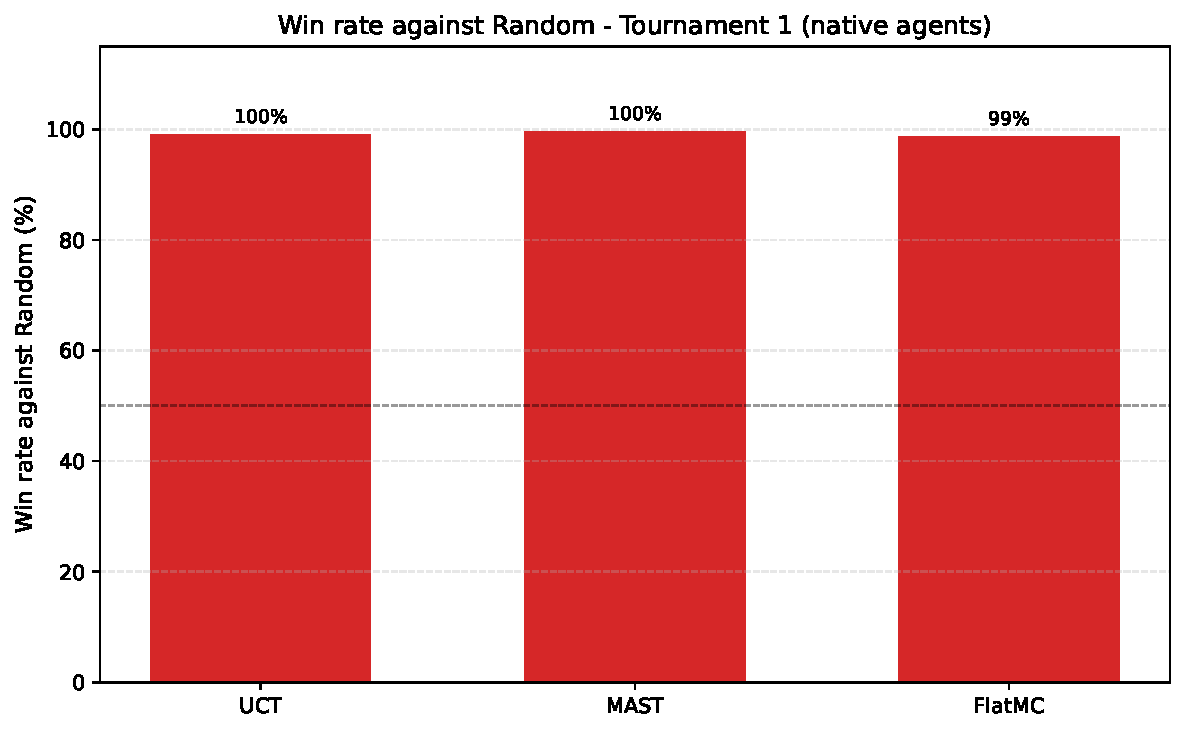
\includegraphics[width=0.95\textwidth]{Sections/5_Ludii/figs/winrate_vs_random_t1.pdf}
    \captionsetup{justification=centering}
    \caption{Win rates of native Ludii agents playing Battleship with unrestricted \textsc{copyContext()}. UCT, MAST, and FlatMC achieve near-perfect win rates against the Random agent, revealing systematic information leakage during simulation.}
    \label{fig:ludii_native_winrate}
\end{figure}

% TODO: Replace the placeholder figure path above with the actual experimental figure once results are available.
% The narrative below reflects the expected experimental outcome based on the architecture analysis.

The results are unambiguous. UCT, MAST, and FlatMC all achieve dramatically higher win rates than the Random agent, approaching near-perfect performance in direct matchups. This is the direct signature of information leakage: these agents effectively know the opponent's fleet layout from the very first move, since every \textsc{copyContext()} call hands them a complete map of the board.

The Random agent, which never calls \textsc{copyContext()}, performs at the expected $\approx 0\%$ level against all opponents and cannot exploit hidden information regardless of what the copy contains. This confirms that the performance gap observed in other agents is not due to superior search algorithms or better evaluation functions, but purely to the privileged access to hidden state that \textsc{copyContext()} provides.

\subsection{Quantifying the Leakage Effect}

The magnitude of the effect in Battleship is particularly large because the game's uncertainty is entirely spatial: the opponent's fleet covers 17 cells out of 100, and knowing their exact positions trivially reduces the problem to a deterministic sequence of targeted shots. An agent with full information can sink the entire fleet in exactly 17 moves; an agent under genuine uncertainty must explore the board through trial and error over many more turns.

This makes Battleship an ideal stress test for information leakage: if a framework exposes hidden positional information, its simulation-based agents will detect and exploit it immediately, producing a measurable win-rate gap over agents that cannot access simulations.


%%% 4.4 %%%
\section{Discussion}
\label{sec:ludii_discussion}

\subsection{Consequences for AI Research in Ludii}

The experimental results demonstrate a concrete and serious problem for AI research conducted within Ludii on imperfect-information games. When native agents are used as baselines in such experiments, the results no longer measure genuine reasoning under uncertainty. An agent that appears to perform well may simply be exploiting information it should not have access to.

This has three direct consequences. First, \textbf{win rates become uninterpretable}: a high win rate for UCT over Random does not demonstrate that UCT reasons better under uncertainty; it demonstrates that UCT exploits privileged state information. Second, \textbf{comparisons between agents become unfair}: agents that rely more heavily on simulations will benefit more from the leakage, systematically overstating their advantage over less simulation-intensive approaches. Third, \textbf{algorithm development is undermined}: any imperfect-information algorithm evaluated against native Ludii baselines will be compared against artificially inflated performance figures, making it difficult to assess genuine progress.

\subsection{Consequences for General Game Playing}

The implications extend beyond Battleship. Ludii hosts over one thousand games, a growing fraction of which involve hidden information. GGP competitions that use Ludii as their platform, and research that compares agents across this game library, are both affected whenever hidden-information games are included. The problem is not limited to spatial hidden information: any game that uses \texttt{set Hidden} in its \textsc{.lud} description is subject to the same leakage through \textsc{copyContext()}.

For GGP research in particular, the ability to evaluate agents on a fair and consistent basis across diverse games is fundamental. A framework in which some agents unknowingly access privileged information cannot serve as a reliable platform for this purpose.

\subsection{Why the Problem is Architectural, Not Incidental}

It is important to emphasize that this is not a bug that can be patched by modifying a single line of code. The \textsc{copyContext()} method was designed for perfect-information games, where copying the complete state is both correct and desirable. Introducing player-awareness into this method at the engine level would require either modifying \textsc{copyContext()} to accept a player identifier, which would break backward compatibility with all existing Ludii agents, or introducing a parallel copy mechanism that agents can optionally use for imperfect-information reasoning.

The solution proposed in Chapter~\ref{DeterminizationLayerLudii} takes a third approach: intercepting the copy at the agent level rather than modifying the engine, thereby preserving full backward compatibility while enabling coherent hidden-state reasoning for any agent that opts into the determinization layer.

\subsection{Summary}

This chapter has established three main points. Battleship in Ludii is a well-formed imperfect-information game at the description level, but native simulation-based agents receive full knowledge of hidden ship positions through \textsc{copyContext()}. This leakage is not intentional: it is a structural consequence of an engine designed for perfect-information games. Empirically, the leakage produces near-perfect win rates for simulation-based agents against non-simulating baselines, confirming that the problem is systematic and measurable. These observations motivate the determinization layer introduced in the next chapter, which replaces raw context copies with coherent hypothetical states that respect the hidden-information constraints declared in the game description.
